\documentclass{standalone}
\usepackage[utf8]{inputenc}
\usepackage{pgfplots}
\DeclareUnicodeCharacter{2212}{−}
\usepgfplotslibrary{groupplots,dateplot}
\usetikzlibrary{patterns,shapes.arrows}
\pgfplotsset{compat=newest}
\begin{document}
% This file was created by tikzplotlib v0.9.8.
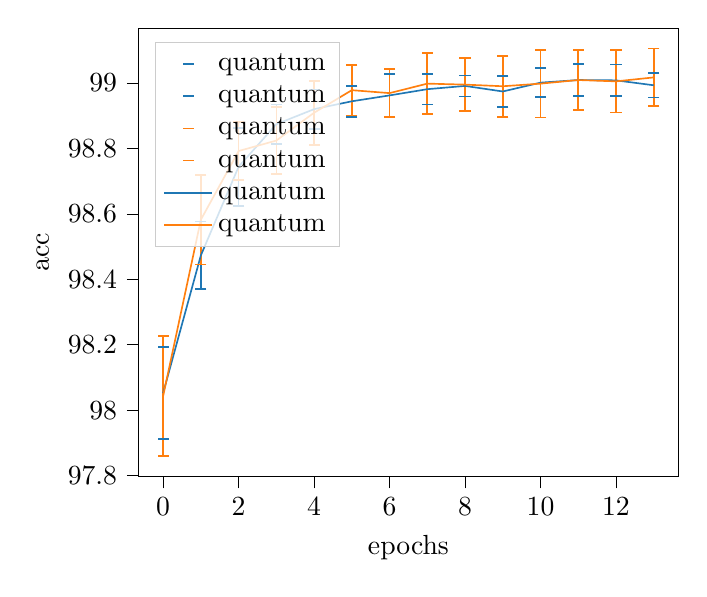
\begin{tikzpicture}

\definecolor{color0}{rgb}{0.12156862745098,0.466666666666667,0.705882352941177}
\definecolor{color1}{rgb}{1,0.498039215686275,0.0549019607843137}

\begin{axis}[
legend cell align={left},
legend style={
  fill opacity=0.8,
  draw opacity=1,
  text opacity=1,
  at={(0.03,0.97)},
  anchor=north west,
  draw=white!80!black
},
tick align=outside,
tick pos=left,
x grid style={white!69.0196078431373!black},
xlabel={epochs},
xmin=-0.65, xmax=13.65,
xtick style={color=black},
y grid style={white!69.0196078431373!black},
ylabel={acc},
ymin=97.7968521662358, ymax=99.1673938889913,
ytick style={color=black}
]
\path [draw=color0, semithick]
(axis cs:0,97.9106635220476)
--(axis cs:0,98.1933364779524);

\path [draw=color0, semithick]
(axis cs:1,98.3697478813777)
--(axis cs:1,98.5762521186223);

\path [draw=color0, semithick]
(axis cs:2,98.6249034005523)
--(axis cs:2,98.8630965994477);

\path [draw=color0, semithick]
(axis cs:3,98.8141334818116)
--(axis cs:3,98.9338665181884);

\path [draw=color0, semithick]
(axis cs:4,98.859667587484)
--(axis cs:4,98.980332412516);

\path [draw=color0, semithick]
(axis cs:5,98.8966291228707)
--(axis cs:5,98.9913708771293);

\path [draw=color0, semithick]
(axis cs:6,98.8964561215673)
--(axis cs:6,99.0275438784327);

\path [draw=color0, semithick]
(axis cs:7,98.9342132497388)
--(axis cs:7,99.0277867502612);

\path [draw=color0, semithick]
(axis cs:8,98.9589219701353)
--(axis cs:8,99.0230780298647);

\path [draw=color0, semithick]
(axis cs:9,98.9268406955098)
--(axis cs:9,99.0211593044902);

\path [draw=color0, semithick]
(axis cs:10,98.957079617488)
--(axis cs:10,99.044920382512);

\path [draw=color0, semithick]
(axis cs:11,98.9605335167358)
--(axis cs:11,99.0574664832642);

\path [draw=color0, semithick]
(axis cs:12,98.959461355602)
--(axis cs:12,99.0565386443981);

\path [draw=color0, semithick]
(axis cs:13,98.9555700654556)
--(axis cs:13,99.0304299345444);

\path [draw=color1, semithick]
(axis cs:0,97.8591495172702)
--(axis cs:0,98.2268504827299);

\path [draw=color1, semithick]
(axis cs:1,98.4452666829189)
--(axis cs:1,98.7187333170811);

\path [draw=color1, semithick]
(axis cs:2,98.7034788160947)
--(axis cs:2,98.8805211839053);

\path [draw=color1, semithick]
(axis cs:3,98.7215109761975)
--(axis cs:3,98.9264890238025);

\path [draw=color1, semithick]
(axis cs:4,98.8113834030505)
--(axis cs:4,99.0066165969495);

\path [draw=color1, semithick]
(axis cs:5,98.9005661572696)
--(axis cs:5,99.0554338427304);

\path [draw=color1, semithick]
(axis cs:6,98.8954540959672)
--(axis cs:6,99.0425459040328);

\path [draw=color1, semithick]
(axis cs:7,98.905285384108)
--(axis cs:7,99.090714615892);

\path [draw=color1, semithick]
(axis cs:8,98.9139753124042)
--(axis cs:8,99.0760246875958);

\path [draw=color1, semithick]
(axis cs:9,98.8968334824092)
--(axis cs:9,99.0831665175908);

\path [draw=color1, semithick]
(axis cs:10,98.8948690153252)
--(axis cs:10,99.1011309846749);

\path [draw=color1, semithick]
(axis cs:11,98.9164311067366)
--(axis cs:11,99.1015688932633);

\path [draw=color1, semithick]
(axis cs:12,98.9098947950951)
--(axis cs:12,99.1001052049049);

\path [draw=color1, semithick]
(axis cs:13,98.9289034620431)
--(axis cs:13,99.105096537957);

\addplot [semithick, color0, mark=-, mark size=2, mark options={solid}, only marks]
table {%
0 97.9106635220476
1 98.3697478813777
2 98.6249034005523
3 98.8141334818116
4 98.859667587484
5 98.8966291228707
6 98.8964561215673
7 98.9342132497388
8 98.9589219701353
9 98.9268406955098
10 98.957079617488
11 98.9605335167358
12 98.959461355602
13 98.9555700654556
};
\addlegendentry{quantum}
\addplot [semithick, color0, mark=-, mark size=2, mark options={solid}, only marks]
table {%
0 98.1933364779524
1 98.5762521186223
2 98.8630965994477
3 98.9338665181884
4 98.980332412516
5 98.9913708771293
6 99.0275438784327
7 99.0277867502612
8 99.0230780298647
9 99.0211593044902
10 99.044920382512
11 99.0574664832642
12 99.0565386443981
13 99.0304299345444
};
\addlegendentry{quantum}
\addplot [semithick, color1, mark=-, mark size=2, mark options={solid}, only marks]
table {%
0 97.8591495172702
1 98.4452666829189
2 98.7034788160947
3 98.7215109761975
4 98.8113834030505
5 98.9005661572696
6 98.8954540959672
7 98.905285384108
8 98.9139753124042
9 98.8968334824092
10 98.8948690153252
11 98.9164311067366
12 98.9098947950951
13 98.9289034620431
};
\addlegendentry{quantum}
\addplot [semithick, color1, mark=-, mark size=2, mark options={solid}, only marks]
table {%
0 98.2268504827299
1 98.7187333170811
2 98.8805211839053
3 98.9264890238025
4 99.0066165969495
5 99.0554338427304
6 99.0425459040328
7 99.090714615892
8 99.0760246875958
9 99.0831665175908
10 99.1011309846749
11 99.1015688932633
12 99.1001052049049
13 99.105096537957
};
\addlegendentry{quantum}
\addplot [semithick, color0]
table {%
0 98.052
1 98.473
2 98.744
3 98.874
4 98.92
5 98.944
6 98.962
7 98.981
8 98.991
9 98.974
10 99.001
11 99.009
12 99.008
13 98.993
};
\addlegendentry{quantum}
\addplot [semithick, color1]
table {%
0 98.043
1 98.582
2 98.792
3 98.824
4 98.909
5 98.978
6 98.969
7 98.998
8 98.995
9 98.99
10 98.998
11 99.009
12 99.005
13 99.017
};
\addlegendentry{quantum}
\end{axis}

\end{tikzpicture}

\end{document}